\documentclass[14pt,fleqn]{extarticle}
\RequirePackage{prepwell}

\previewoff


\begin{document} 
\begin{skill}
    \begin{narrow}
         \textcolor{blue}{Ellipse Basics}
    \end{narrow}
    
    \reason 
    
    \begin{center}
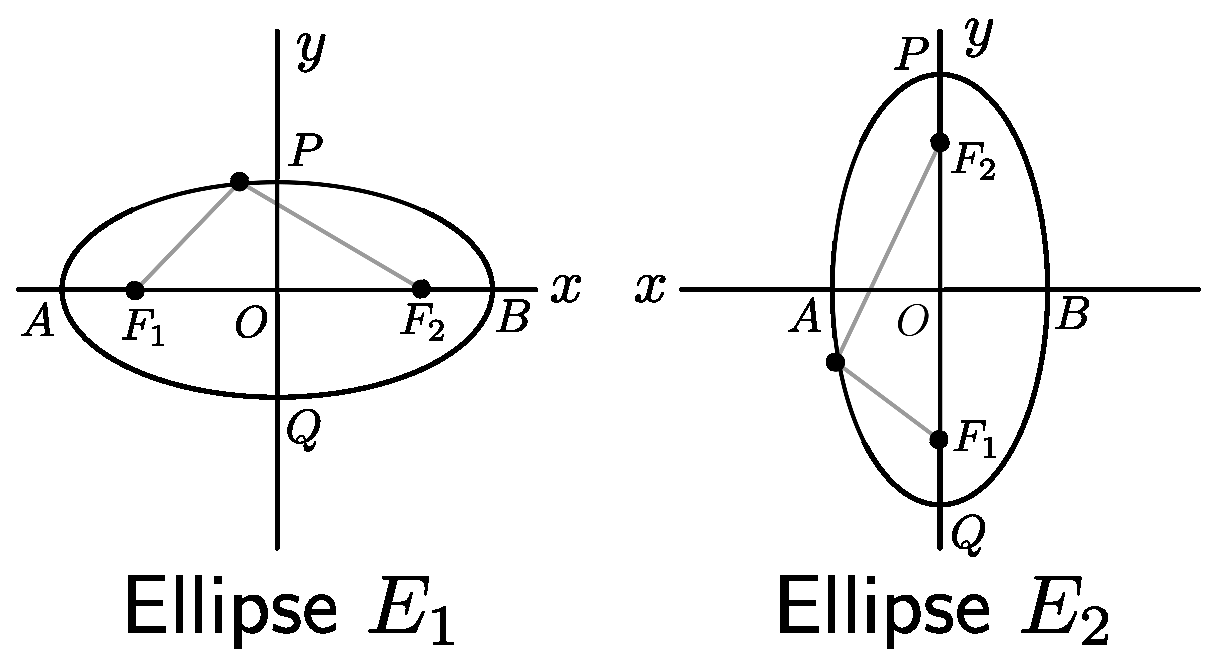
\includegraphics[scale=0.4]{figure.eps}
\end{center}

An ellipse is the locus of all points the sum of whose distances 
from two fixed points (the foci) is constant \newline 

The following are common to $E_1$ and $E_2$ 
\begin{center}
  \begin{tabular}{Nl}
   \toprule
        & Meaning \\
   \midrule 
   O & The center. When $F_1,F_2$ and $O$ \\
   & coincide, then we have a circle \\ 
    \midrule 
    F_1 \text{ and } F_2 & The foci. Always on the major-axis \\
    \midrule
    \pi\cdot ab & Area of the ellipse \\
    \bottomrule
  \end{tabular}
\end{center}

And the following are the \underline{differences}
\begin{center}
  \begin{tabular}{lNNN}
   \toprule
        &  \text{Ellipse }E_1 & \text{Ellipse }E_2 & \text{Note} \\
   \midrule 
   Major axis & AB & PQ & \\
    \midrule 
    Minor axis & PQ & AB &\\
    \midrule
    Vertices & A, B & P, Q & \\
    \midrule 
    Equation & \frac{x^2}{a^2} + \frac{y^2}{b^2} = 1 & \frac{x^2}{b^2} + \frac{y^2}{a^2} = 1 & O = (0,0) \\
    & & & a > b \\
    \midrule 
    Parametric & x = a\cos\theta & x = b\cos\theta & O = (0,0)\\
    & y = b\sin\theta & y = a\sin\theta & a > b\\
    \bottomrule
  \end{tabular}
\end{center}

    
\end{skill}
\end{document} 